\chapter{Requirements, Impacts and Constraints}
\label{ch:3}

More than accuracy is judged by a system that responds to people describing painful experiences. It should function with the hardware that a student team owns, it should not use the data it learns from in a way that violates the licence of the data, it should not misuse anything a person types to it, and it should never pretend to be providing any kind of help that it is not qualified to provide. This chapter outlines the requirements that were designed to address those demands and the potential impact the system may have on people and the environment, as well as the ethical considerations imposed upon the system, what standards are adhered to, and how the project was planned and the risks and costs managed.

\section{Final Specifications and Requirements}
\label{sec:3.1}

This work needed to meet both technical and methodological requirements. Technically, two models needed to run in parallel on a single consumer graphics card and respond within a few seconds, one a RoBERTa-base classifier that reads the user's message and returns the three most likely emotions along with the words that led to the decision, and another 3.8-billion-parameter instruction model, quantised to 4 bits, that selects one of those emotions and writes the reply. Methodologically, all design decisions were required to be decided by measuring on the same held-out conversations and all numbers used in this thesis had to be reproducible from saved outputs. The following requirements were established prior to the final round of development and were not changed after that round; each is stated in a way that it may readily be checked by measurement.

\subsection{Functional Requirements}

\begin{itemize}
  \item \textbf{}\textbf{Emotion detection from the users' actual words:} the emotion is read from the message the user actually writes, there are 32 categories of the EmpatheticDialogues \cite{sharma2020epitome}
  \item \textbf{Candidate emotions, not a single guess:}The detector returns a number of probable emotions with a confidence percentage each.
  \item \textbf{Visible emotional decision:} Each response contains all the candidates, the emotion and the words behind it.
  \item \textbf{Guided generation:} The generator is given wording for the emotion chosen.
  \item \textbf{Response rules: }each response validates the emotion, poses a single question and maintains a word limit of 120.
  \item \textbf{Multi-turn conversation: }the parts feature a conversation that lasts multiple turns and the parts are able to register when the emotion shifts.
\end{itemize}
\subsection{Non-Functional Requirements}

\begin{itemize}
  \item \textbf{Hardware budget:} all the system is based on one consumer GPU equipped with 8 GB memory \cite{devlin2019}.
  \item \textbf{Privacy by locality:} no user message has to leave the device.
  \item \textbf{Response time: }a few seconds is the response time on that hardware.
  \item \textbf{}\textbf{Reproducibility:} Numbers may be reproduced from outputs saved, using fixed seeds.
  \item \textbf{Inspectability: }the ability to replace and test each component individually.
  \item \textbf{Cost:} Only open models, datasets and free tiers of services are used.
\end{itemize}
\subsection{Hardware and Software Requirements}

\textbf{Hardware specifications:} All training, generation and benchmarking were performed on a single machine equipped with one of the NVIDIA GeForce RTX 4060 GPUs with 8 GB of video memory, 16 GB of system memory and a solid-state disk for the model cache, and was running Windows 11. That card is just a necessary part of the card, not a restriction --- the design goal was a system that a counselling service can run on a typical computer. It defines the upper limit of the design it is required to work under, as the detector, the quantised generator and their activations must all fit into 8G, and it is the hardware used to measure the 3.40Gb peak memory and 4.17s per reply time in Chapter 5. 

\textbf{Software requirements:} the system was implemented in Python 3.10 using PyTorch 2.5.1 with CUDA 12.1 \cite{liu2019roberta} and Hugging Face Transformers 5.16.1 \cite{qwen2024} to provide the pre-trained encoder and the instruction-tuned generator. Without using PEFT for low-rank adaptation and bitsandbytes for 4-bit NF4 quantisation, the generator wouldn't fit in 8 GB, hence it was fine-tuned using those. To perform the paired tests and classification metrics, SciPy \cite{abouelenin2025phi4mini} and scikit-learn \cite{dettmers2023qlora} were used; sentence-transformers \cite{hu2022lora} for the retrieval baseline; WASSA 2024 empathy classifier \cite{li2024emotioncot} and OpenRouter and Groq APIs for the judges. The demonstration is based on Gradio and the human study Google Forms; the specific versions of the libraries used are provided in the appendix.

\subsection{Data Requirements}

For the work, the data had to be conversational with fine-grained emotions, and EmpatheticDialogues provides 23,144 conversations and 88,687 utterances, each conversation with one of 32 emotion labels, divided into 17,839 conversations for training, 2,763 for validation and 2,542 for testing \cite{sharma2020epitome}. 17780 pairs of text are used to train the detector, which is being trained on the first message of each conversation, the text it receives in use. Quality of reply is evaluated on 64 stratified conversations provided by every system, out of a set of 300 held-out conversations. The corpus is made available in a research licence \cite{belay2025} that is non-commercial. 

\subsection{Design Constraints}

There were a number of constraints that influenced the design, rather than just restricting it. The 8 GB memory budget precludes an unquantised generator and any model larger than 8 billion parameters, hence the quantisation of the generator and the design of the detector to be small. The dataset assigns one emotion label to each conversation, but a conversation may contain multiple emotions simultaneously, which makes the detection accuracy against the reference label less than perfect. The free evaluation services limit the number of requests per day, so we were able to only evaluate 64 conversations per system using the AI-judge and the human study was limited to a short questionnaire due to the availability of volunteers. The project also required one GPU to be shared by three members, and a fixed academic deadline, so experiments were prioritized by cost, with cheap local experiments being done first, and rate-limited experiments only being done if a design had already been proven to be worth the time and money. 

\section{Societal Impact}
\label{sec:3.2}

\subsection{Potential Benefits}

The system is designed for the time when there is a need to be listened to and no trained listener is available. It is designed to have six benefits.

\textbf{Privacy for people who won't talk to a cloud service:} both models operate on the user's own machine, which means that a disclosure about grief, loneliness or fear never leaves the user's machine, which for many people is the difference between writing the message and not writing it at all.

\textbf{A listener available at every hour: }distress doesn't have office hours, and a locally hosted system answers at three in the morning, on a holiday or after the counselling centre has closed.

\textbf{It's a first step towards professional help:} it's not a therapist and should not be used to replace a therapist, but it can start the first conversation and make it feel less like a big step to reach out to a counsellor.

\textbf{Low cost to the institutions that need it most: }it can be hosted on a single computer at a counselling service, a small clinic or a helpline without any per-message cost. In Bangladesh, where there are few mental-health professionals and private counselling is out of the reach of the majority of students, the cost of access is as important as the nature of the response.

\textbf{A way to avoid stigma: }many people will type a worry that they would never say out loud to a relative or a doctor.

\textbf{Replies that can be checked before viewing: }the emotion behind each turn is written down, and a supervisor can check it, and a safeguard can prevent the person from viewing the reply. There is no model to inspect in a single end-to-end model. 

\subsection{Risks and Limits of Use}

Three risks are explicitly stated because a sounding system can be trusted more than it is warranted.

\textbf{Overuse of the substitution call: }someone in distress may continue to speak to the machine rather than reaching out to someone who can help. Since there is no crisis filter, and the emotion categories do not include suicidal thoughts, it should never be deployed as a mental-health service, any use should have a reviewed filter, a referral path and a visible helpline number \cite{hu2022lora}.

\textbf{Wrong or shallow empathy: }detector's first guess is correct 50.3\% of the time, reply mentions the user's actual emotion 36.7\% of the time, and replies based on the wrong emotion can be dismissive. With three candidates passing, that cost is reduced, but for one person at one time the risk is very real.

\textbf{Cultural and linguistic fit:} EmpatheticDialogues has been developed by English speaking crowdworkers \cite{sharma2020epitome} and there are language differences in the expression of feelings; therefore, data and evaluation in Bangla would be required before use in Bangladesh.

To sum up: the design provides an institution with privacy, affordability, an auditable emotional decision, and pays for it by providing replies that are not rated better than one model's by the AI. 

\section{Environmental Impact}
\label{sec:3.3}

The environmental impact of this work is the electricity consumed by training and testing the models, which is minimal due to the fact that each model is small. All training and local inference was performed on a single RTX 4060 rated for 115 W of board power \cite{devlin2019}. When measuring the power consumption (rated power times GPU hours, which overestimates the actual draw), the last detector required approximately 0.017 kWh, while the RoBERTa-large alternative required approximately 0.124 kWh. The most significant loads were generated for fourteen configurations with 300+ conversations each, and fine-tuning for a few kilowatt hours, which would correspond to a desktop running for a few days. No CloudGPU is rented, nothing is trained from scratch.,The design also has a direct environmental impact in use: Within statistical error the system is as good as a single model with 1.9 times its parameters, but with 38\% less GPU memory, so a service that would otherwise require a data-centre GPU can be run on a mid-range consumer card, and because everything is local, no message need be sent to the data centre, and back. Also no new hardware was purchased, and the 8 GB limit was deliberately made so that no new hardware was required. 

\section{Ethical Issues}
\label{sec:3.4}

When someone is upset, a response comes with responsibilities that are not accounted for in an accuracy score. This project has been influenced by 7 of them.

\textbf{Safety and scope}

The system is meant for supportive listening in low-risk conversations, and is neither a therapeutic nor a diagnostic nor a crisis service. The most dangerous case is when the user says that he/she is thinking about killing themselves; there is no category for ``suicidal ideation'' in the 32 categories of EmpatheticDialogues \cite{sharma2020epitome} and thus the detector can't even represent such a message. When tested, a response of `I want to die' was interpreted as \textit{afraid }(45\%) and \textit{terrified }(28\%), and the response was warm, but no crisis service was mentioned, and commercial assistants responded predominantly with helpline information. It is not sufficient by itself as World Health Organization guidelines call for understanding and accurate information on where to obtain assistance \cite{hu2022lora}. Here mitigation is limited to the interface, stating that the system is an unmonitored student project, and providing crisis services. There is a pre-generation crisis filter which is crucial before deployment and the decoupled design makes it possible to add, as the emotion is determined prior to any text being written.

\textbf{Clinical Responsibility}

The system generates texts that seem like emotional support, but no one clinically qualified responds. Three commitments follow: it will never be marketed to a user as a counsellor, therapist or helpline; the emotional decision behind each response is recorded and can be audited; and prior to deployment it must be reviewed by a qualified professional, operated with a crisis filter, and a referral path and have a named person accountable for its operation.

\textbf{Protection of personal data and privacy}

All models were built and tested using the publicly available EmpatheticDialogues dataset and no personal data was gathered, just the text of the dataset and resulting generated responses submitted to judge services. Both models operate locally, meaning that a deployed instance does not require a disclosure to an external provider, and the demonstration stores conversation history by keeping it in memory only, thus not writing it to disk.

\textbf{Human Evaluation}

The human evaluation in Chapter 5 presents the results of a rating of responses to 8 short situations by volunteers, predominantly students with a few faculty members. Participation is voluntary and anonymous, no name or email addresses are collected and participants are told beforehand how long the activity will take (15 minutes) and warned that some of the scenarios involve stressful experiences, and that they can stop anytime they want. Each answer has its own system, and the order in which the answers were given is counterbalanced, so no one can be directed towards the authors' system.

\textbf{Data and Model Licensing}

EmpatheticDialogues has been published under CC BY-NC 4.0 \cite{belay2025} which stipulates that the detector trained on it must be attributed and cannot be incorporated into a commercial product. The Phi-4-mini-instruct model is licensed under MIT, the RoBERTa baselines are licensed under Apache-2.0, and the Gemma-3 candidate has the following license: Google's Gemma Terms of Use \cite{lewis2020rag}. There is no licence for the WASSA empathy model and it is used for evaluation purposes only with credit to the authors.

\textbf{Bias and Fairness}

EmpatheticDialogues is an English-only corpus written by crowdworkers and, thus, detection accuracy, as well as the appropriateness of the replies is not guaranteed to transfer to Bangladesh users. The evaluation itself is imbued with its own bias: the acknowledgement check is one that searches for phrases such as ``I'm sorry'', which are appropriate to negative emotions and to under-credit good responses to positive ones -- it is never used alone, but in conjunction with the AI-judge panel, the empathy classifier and the human study.

\textbf{Research Integrity}

A failure was not deemed a result and negative findings are reported fully: retrieval augmentation, the fine-tuned generator, the Gemma-3 candidate, the larger detector and the result that our superiority over a single, same-size model in terms of rule adherence was not borne out by the correction. If a configuration error was detected in the finely-tuned base line, it was re-trained and all results affected were replaced -- the error was not obscured. All the figures used in this thesis are recreated from saved results using scripts in the project repository.

\section{Standards}
\label{sec:3.5}

There are no engineering standards for an empathetic dialogue system, so the project was conducted following the published practice which applies to the components thereof. All data and models are used under their respective licenses and EmpatheticDialogues is only available for non-commercial research. The response rules are in line with guidance for supportive conversation: using the emotional-reaction mechanism of the EPITOME framework \cite{who2022report} for the "acknowledge the feeling" rule, and the "single question" rule in line with counselling guidance against the question-answer trap \cite{reimers2019sbert}. The classifier is taken from the WASSA 2024 shared task \cite{wu2025traits} and the AI-judge evaluation is performed according to the accepted practice: blind (without identifying the authors of the works), anchored (with a strict rubric), temperature 0 (the AI-judge is not allowed to deviate from the rubric) and judges from unrelated developers \cite{koga2023implicit}. Paired tests with correction for multiple comparisons (Section 5.4.1) are used for statistical claims. The one requirement it fails to meet is the requirement of the World Health Organization, which has no crisis safeguard and should not be used as a mental-health service \cite{hu2022lora}. The work is also in accordance with the academic conduct requirements of BRAC University: sources cited, results of the team's own runs reported, errors reported and not removed. 

\section{Project Management Plan}
\label{sec:3.6}

The project was conducted by a team of three for 9 months with one machine with a GPU, divided into three, and a fixed academic deadline. The work was not conducted in a linear sequence, but rather in a series of overlapping phases, evaluation, writing and experimentation, so that if a result proved to be one that challenged an assumption, it could be integrated without halting the other processes. An iterative, evidence-gated approach was used for development. All the design alternatives were tested, using the same 300 conversations held out and scored using the same measures; only if the numbers supported the design alternative were they kept. Cheap local measures served as a first gate, and the rate-limited AI judges and human study were used only for candidates that passed the first gate. The work is split into 5 phases as illustrated in the Gantt chart in figure 3.1. The dates are based on the dates of manufacture of each set of artefacts and the chart illustrates what occurred.

\begin{itemize}
  \item \textbf{Phase 1 - Background study and candidate selection (January to May 2026):} the problem was defined, the literature reviewed, and first detectors and generators trained on GoEmotions.
  \item \textbf{Phase 2 - Move to EmpatheticDialogues (June 2026): }The initial comments were found to be inappropriate for a conversational system, and the work was restarted with a conversational corpus, resulting in the first detector on the new corpus.
  \item \textbf{ Phase 3 - Evaluation of the initial pipeline (July to August 2026): }the first complete pipeline was measured against zero-shot, fine-tuned and single-model baselines with an AI-judge panel, an empathy classifier and paired tests.
  \item \textbf{Phase 4 - Design adjustment (August to September 2026):} that evidence drove the corrected detector, the generator comparison, the two-stage emotion selection, per-emotion guidance and attention cues, giving the final system.
  \item \textbf{} \textbf{Phase 5 - Validation, agent and writing (September 2026):} robustness checks, multi-turn agent, human evaluation and this report.
\end{itemize}
\begin{figure}[htbp]
\centering
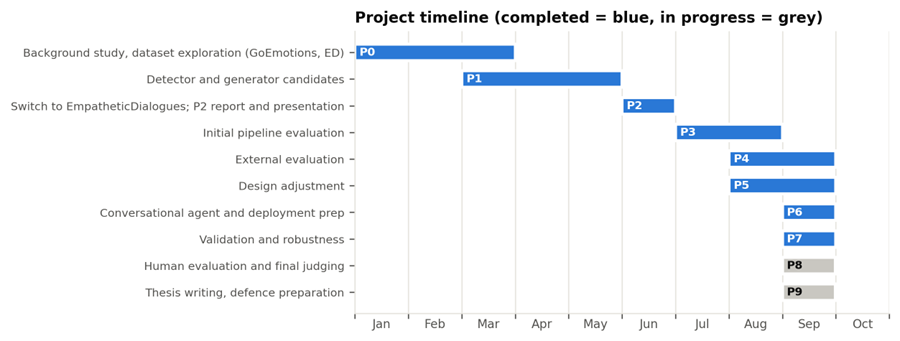
\includegraphics[width=0.95\linewidth]{figures/ch3_fig1.png}
\caption{Project timeline}
\label{fig:3.1}
\end{figure}

\section{Risk Management}
\label{sec:3.7}

Risks were documented if any of the experiments behaved in an unusual manner or if a phase was reexamined and assigned a level of probability and severity for the resulting effects, schedule or user safety. In most cases the mitigation was structural (not procedural), that is, by implementing an automatic check, a fixed seed or a pinned version, the same failure could not occur undetected. In total twelve risks were identified, eight of which happened, two of which were averted and two of which haven't yet been resolved. Three entries made adjustments to the way the project works.

\begin{itemize}
  \item \textbf{Silent technical failure:} the design queried the detector about the attention weights that it was using to retrieve the words that it predicted, but the default attention implementation on the library fails to return anything without throwing an error, meaning cue extraction reverted to simple text splitting, which appeared to be working correctly. If left undiscovered, the thesis would have been a description of a mechanism that wasn't running. This was changed and now an automatic check stops execution when the weights are missing.
  \item \textbf{Validity of the results:} The original detector had been trained on situation descriptions and then used on the user's own messages but achieved lower accuracy (56.9\% to 48.2\%) and the accuracy on the real input, so it was retrained. A RoBERTa-large run, which ran into a missing warmup, went astray to 5.0\%, but it was determined and repeated to 53.0\% instead.
  \item \textbf{External services dependence:} the AI judges were third-party services that were not under the control of the teams, with several candidates being retired or restricted during the project. The systems that were 'fixed' on the two systems that remained available throughout are scored by the same judges, and rate limited work was split between two accounts, with every emotion represented in both halves.
\end{itemize}
There are 2 risks open. Collecting judge scores and items for human evaluation will be discarded if the design changes at the last minute, and the improvement due to the repetition penalty is left for later. Moreover, apart from interface disclaimers, the system does not have a safeguard for disclosure of suicidal thinking that needs to be addressed prior to deployment (Section 3.4).

\section{Economic Analysis}
\label{sec:3.8}

The project has been designed as close to cost-free as possible, as the constraint of a student team is the one that a small clinic faces. All models are openly released, all libraries open source, the data set is freely available for research, the judges are free-tier, and the human study is based on a free questionnaire service -- direct spending is only electricity, Internet access and a GPU workstation already owned by the team. Energy is equally small: at the card's rated 115 W, fine-tuning the final detector used about 0.017 kWh in 8.8 minutes and RoBERTa-large about 0.124 kWh in 64.7 minutes so the cost of training is negligible.

\subsection{Cost-Benefit of the Main Design Choices}

\begin{itemize}
  \item \textbf{Where the more cost-effective choice won: }RoBERTa-large is 2.9 points more accurate than RoBERTa-base but 2.8 times larger with 7.4 times more training time, and did not affect any reply quality measure when replacing RoBERTa-base in the final system. The same training took 43 minutes of GPU time for fine-tuning, but only achieved a 22.3\% hit rate of the three rules; the instruction-tuned model had no training required and attained 60.0\%.
  \item \textbf{Where it did not:} a single Qwen2.5-7B model beats our pipeline on rule adherence, empathy-classifier score and judge-empathy, so if you only look for quality, using it is better; but if you compare peak memory consumption on the same GPU, our system uses 38\% less and achieves 97.5\% of the overall judge score of that model.
  \item \textbf{}         \textbf{Evaluation method:} The human study confirms those free-tier AI judges -- they are not replacing humans, they are paid roughly USD 6 per hour in one published study and the human study evaluates several hundred of them at no cost.
\end{itemize}